\begin{frame}{Effect on Solution Length - Metric 1}

\begin{itemize}
\item Solution length difference between the condition (Y) and the control (N) groups \textbf{is not statistically significant}
\end{itemize}
\begin{figure}[tpb]
  \centering
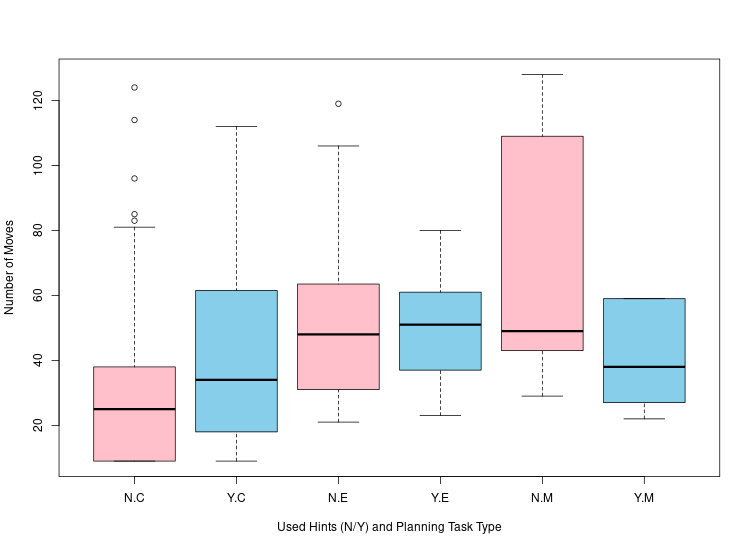
\includegraphics[width=0.8\columnwidth]{../img/lenbytype.png}
  \label{fig:lenbytype}
\end{figure}

\end{frame}

\begin{frame}{Moving the User's Solution Closer to the Optimal Solution - Metric 2}

\begin{itemize}
\item Solution length difference to the cost optimal solution between the condition (Y) and the control (N) groups \textbf{is not statistically significant}
\end{itemize}
\begin{figure}[tpb]
  \centering
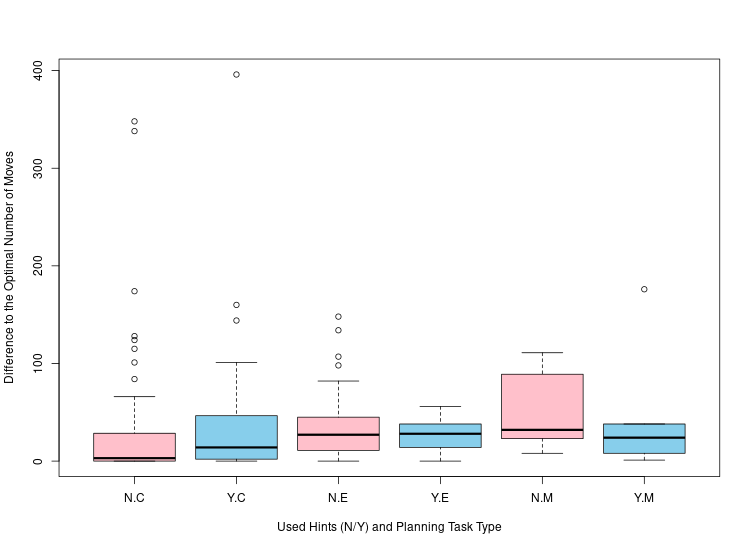
\includegraphics[width=0.7\columnwidth]{../img/lenoptbytype.png}
  \label{fig:lenoptbytype}
\end{figure}

\end{frame}

\begin{frame}{Moving the User's Solution Closer to the Optimal Solution - Metric 3}

\begin{itemize}
\item The latest times until the landmarks are achieved between the condition (Y) and the control (N) groups \textbf{is not statistically significant}
\end{itemize}
\begin{figure}[tpb]
  \centering
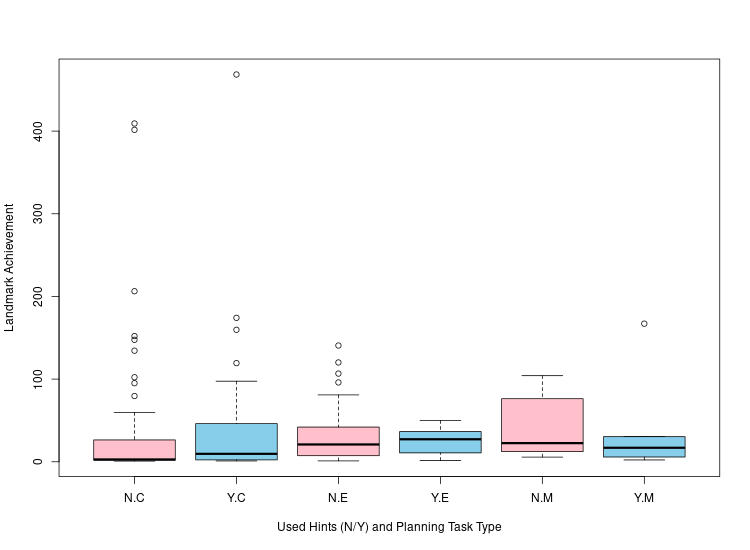
\includegraphics[width=0.7\columnwidth]{../img/achbytype.png}
  \label{fig:achbytype}
\end{figure}

\end{frame}

\begin{frame} {Moving the User's Solution Closer to the Optimal Solution - Metric 4}
\begin{itemize}
\item The number of times landmarks are lost and regained between the condition (Y) and the control (N) groups \textbf{is not statistically significant}
\end{itemize}
\begin{figure}[tpb]
  \centering
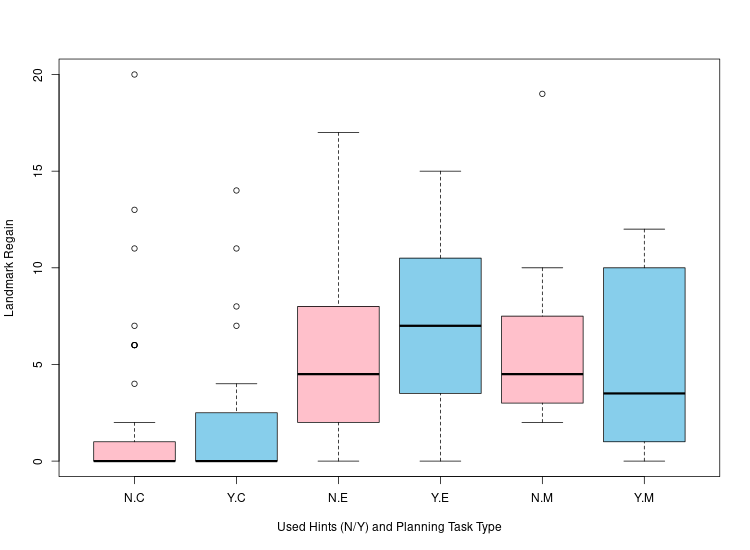
\includegraphics[width=0.7\columnwidth]{../img/regainbytype.png}
  \label{fig:regainbytype}
\end{figure}
\end{frame}